% !TeX root = ../main.tex
\graphicspath{{figures/}}

\chapter{Numerical Methods}

\section{Chebyshev collocation method}
Linear stability analysis is performed by solving the governing equations, the Orr-Sommerfeld equation (\ref{eq:osn}) when considering viscosity effects, and the Rayleigh equation (\ref{eq:rn}) for inviscid assumptions, along with the boundary conditions. The spectral collocation method with Chebyshev polynomials is used to discretize the eigenvalue problem in the vertical direction. 

The concept of the spectral methods implies that unknown functions in the governing equations are expanded using a series expansion, which we chose Chebyshev polynomials of the first kind as the basis functions. Chebyshev polynomials are defined on the interval $\zeta\in[-1,1]$, and the $n$-th Chebyshev polynomial is defined as
\begin{equation}
    T_n(\zeta)=\cos(n\cos^{-1}(\zeta)).
\end{equation}
The unknown functions shall be represented with the Chebyshev polynomials. To implement the Chebyshev polynomial, the physical domain $z\in[-h,0]$ is mapped to the computational domain $\zeta\in[-1,1]$ via coordinate transform
\begin{equation}
    \zeta=\frac{2z}{h}+1,\quad -h\leq z\leq 0.
\end{equation}
In the computational domain, the eigenfunction $\phi$ is expanded using the Chebyshev expansion
\begin{equation}
    \phi(\zeta) =\sum _{n=0}^{N} a_{n} T_{n}(\zeta),
\end{equation}
where $N$ represents the $N$-th Chebyshev polynomial and $a_n$ is the coefficient of the series. Coefficient $a_n$'s replace $\phi(\zeta)$'s as  unknown variables to be solved, with the difference that $a_n$'s are independent of $\zeta$. The derivatives of $\phi(\zeta)$ in the vertical direction are also represented in expanded form, by using chain-rule,
\begin{equation}
    \frac{d^{j} \phi ( \zeta )}{dz^{( j)}} =\left(\frac{2}{h}\right)^{j}\sum _{n=0}^{N} a_{n} T_{n}^{(j)}( \zeta ).
\end{equation}
Here the $(j)$-th order derivative with respect to $\zeta$ of the Chebyshev polynomial $T_{n}^{(j)}( \zeta )$ is involved, and an advantage of the Chebyshev polynomial is that its derivatives can be derived recursively using lower order terms. As stated in Schmid \& Henningson (2001) \cite{RN9},
\begin{equation}
\begin{array}{l}
\displaystyle T_{0}^{( j)}( \zeta ) =0,\quad T_{1}^{( j)}( \zeta ) =T_{0}^{( j-1)}( \zeta ) ,\quad T_{2}^{( j)}( \zeta ) =4T_{1}^{( j-1)}( \zeta ) ,\\
\displaystyle T_{n+1}^{( j)}( \zeta ) =2(n+1)T_{n}^{( j-1)}( \zeta ) +\frac{n+1}{n-1} T_{n-1}^{( j)}( \zeta ) \quad n\geq 2.
\end{array}
\end{equation}
By applying the above relations, the derivatives of $\phi(\zeta)$ can be replaced by linear combinations of $T_{n}( \zeta )$, so that the problem is now a linear algebraic system.

The system is discretized with the use of the collocation method. We evaluate the Chebyshev polynomials at chosen locations, with the restriction that the governing equations be satisfied at these discrete collocation points $(\zeta_1,\zeta_2,...,\zeta_{M-1})$, defined as
\begin{equation}
    \zeta_m=\cos(\frac{\pi m}{M}), m = 1,2,...,M-1.
\end{equation}
This distribution of points is known as the Gauss-Lobatto points and is chosen to minimize the effect of Runge's phenomenon. 

Instead of applying governing equations to the boundaries, we replace them with the boundary conditions derived in previous sections. Considering viscosity, free surface conditions (\ref{eq:kbc}), (\ref{eq:tbc}), and (\ref{eq:nbc}) are applied at the upper boundary $\zeta=\zeta_0=1$, while free-slip conditions (\ref{eq:bbcfs}) are applied at the lower boundary $\zeta=\zeta_M=-1$. This results in a total of $M+4$ equations determining $N+2$ unknowns, with $N+1$ coefficients of the $N+1$ Chebyshev polynomials and the amplitude of surface elevation $q$. For the system to be exactly determined, we choose $M=N-2$.

For inviscid assumptions, the tangential stress condition (\ref{eq:tbc}) is excluded at the free surface, and the exponential decaying condition (\ref{eq:bbced}) is applied at the lower boundary. With a total of $M+2$ equations and $N+2$ unknown, we can simply set $M=N$, so that the number of collocation points equals the order of Chebyshev polynomial used.

The ODE system is then rearranged into a linear algebraic generalized eigenvalue problem (GEP), in mathematical form $\boldsymbol{Ax}=\omega\boldsymbol{Bx}$, with eigenvalue $\omega=kc$ and eigenvector $\boldsymbol{x}^T=[a_0,a_1,...,a_N,q]$. 

\section{Treatment on infinity boundary}
To perform numerical computation, the infinite boundary is treated by truncating the domain to a finite truncation height $h$, and we derive two different methods of the boundary condition (\ref{eq:bbc1}) at the truncation height. The two treatments are compared in chapter (\ref{ch:results}).

The first treatment is done by replacing the boundary condition (\ref{eq:bbc1}) by the free-slip condition
\begin{equation}
    \left.\frac{\partial u}{\partial z}\right|_{z=-h}=\left.w\right|_{z=-h}=0,
\end{equation}
with the fact that $dU/dz=0$ and normal mode expansion,
\begin{equation}
    \frac{d^2\phi(-h)}{dz^2}=\phi(-h)=0.
    \label{eq:bbcfs}
\end{equation}

Another treatment is that by implementing the condition that at infinity depth, the velocity of the background flow approaches the free-stream velocity $U=1$, and thus $d^2U/dz^2=0$. Asymptotic solutions of the governing equation (\ref{eq:osn}) can be solved analytically, approaching four independent exponential solutions
\begin{equation}
    \phi (z) =C_{1} e^{kz} +C_{2} e^{-kz} +C_{3} e^{\left(\sqrt{k^{2} +ikRe}\right) z} +C_{4} e^{-\left(\sqrt{k^{2} +ikRe}\right) z}.
    \label{eq:bbc2}
\end{equation}
The boundary condition (\ref{eq:bbc1}) states that perturbation velocity vanishes at infinity, thus only decaying solutions in equation (\ref{eq:bbc2}) remains. Considering only the dominant terms, the solution is simplified into $\phi(z)=C_1\exp(kz)$. Therefore at a sufficiently low truncation height $z=-h$, the stream function amplitude became
\begin{equation}
    \phi(-h)=C_1 e^{-kh},
    \label{eq:bbc3}
\end{equation}  
which is the modified boundary condition. To apply this boundary condition to system with the Orr-Sommerfeld equation (\ref{eq:osn}) as governing equation, two boundary condition equations are needed. It is done by deriving the $z$-derivatives of the stream function amplitude
\begin{equation}
\begin{array}{lll}
    \phi_{z}(-h) &= k C_1e^{-kh}&=k\phi\left(-h\right)\\
    \phi_{zz}(-h)&= k^2C_1e^{-kh}&=k^2\phi\left(-h\right),
\end{array}
    \label{eq:bbced}
\end{equation}
so that the exponential solution is applied and satisfied without solving for the constant $C_1$. Under inviscid assumptions, the boundary condition is simply represented by the relation with its first derivative $\phi_{z}(-h) =k\phi(-h)$.

\section{Generalized eigenvalue problem}
Multiple methods can be considered for solving the GEPs, basically done by implementing the MATLAB built-in function \inlinecode{eig}, which by default uses the QZ algorithm to solve the GEPs. A GEP can be converted into a standard eigenvalue problem of the form $\boldsymbol{Cx}=\lambda\boldsymbol{x}$ by inverting either matrix $\boldsymbol{A}$ or $\boldsymbol{B}$, with the premise that the matrices are invertible. However, our boundary conditions and matching conditions without $\omega$ terms generate rows of zeros in the matrix $\boldsymbol{B}$, which causes matrix $\boldsymbol{B}$ to be singular and thus not invertible. Two different methods are used to solve this type of GEP, their convergence of eigenvalue with the increase of matrix size are compared subsequently.

The first method is the QZ algorithm mentioned above. The QZ algorithm was designed by Moler \& Stewart (1973) \cite{RN10} to solve problems with a singular or nearly singular matrix $\boldsymbol{B}$, and no inversions of the matrix $\boldsymbol{B}$ are used when solving for the eigenvalue. While with the advantage of solving most GEPs regardless of the singularity of matrices, the computational time for the QZ algorithm increases significantly with the increase of matrix size.

The second method was mentioned in Schmid \& Henningson (2001) in \cite{RN9}, which the main concept of the method is to make matrix $\boldsymbol{B}$ non-singular, for the GEP to be converted to and solved as a standard eigenvalue problem. It is done by replacing the rows of zeros in matrix $\boldsymbol{B}$ by a complex multiple of its corresponding matrix $\boldsymbol{A}$. This operation doesn't affect the solutions of the original equations but produces additional artificial eigenvalues which originally are undefined. These artificial eigenvalues can easily be located and excluded since they are mapped to a specific location in the complex plane by the chosen complex multiple. With both matrices non-singular, the GEP can be converted into a standard eigenvalue problem, either $(\boldsymbol{B}^{-1}\boldsymbol{A})\boldsymbol{x}=\omega\boldsymbol{x}$ or $(\boldsymbol{A}^{-1}\boldsymbol{B})\boldsymbol{x}=(1/\omega)\boldsymbol{x}$.

balancing

\section{Domain decomposition method} \label{ch:ddm}
The distribution of collocation points is fixed to the Gauss-Lobatto points, which are dense near the boundaries and sparse in between. This is sufficient for most problems, where flow properties vary most abruptly near the boundaries that require more collocation points to resolve the variations. Nevertheless, there are still cases that rapid changes of flow properties occur far from the boundaries, hence accentuating the defect in the collocation method.

In our problem, this issue arises in inviscid cases where the Rayleigh equation (\ref{eq:rn}) has a regular singular point at a point $z_0$ with $U(z_0)=c$. The corresponding real part of this point defines the critical point $z_c$ where $U(z_c)=c_r$. For cases with a small imaginary part of the phase velocity, the singularity locates near the real axis, causing abrupt variations of the eigenfunction near the critical point. To resolve the eigenfunction, dense collocation points are required in the neighborhood around the critical point, which doesn't match the collocation point distribution for critical points far from the boundaries. Consequently, a method that preserves the property of the Gauss-Lobatto points while improving the flexibility of the collocation point method is required.

We introduce the domain decomposition method, which is aimed at resolving the rapid variations of the eigenfunction. This is done by splitting the computational domain into multiple smaller domains, with a set of Gauss-Lobatto points in each domain. The distribution of collocation points is then dense near each boundary of smaller domains, therefore by splitting the computational domain at a specific location the density of distribution of points around it is increased. The boundaries between domains are defined by sufficient matching conditions, for inviscid problem the matching condition denotes the continuity of eigenfunction and its first derivative,
\begin{equation}
    \phi _{( k) ,-} =\phi _{( k+1) ,+} ,\quad \frac{d\phi _{( k) ,-}}{dz} =\frac{d\phi _{( k+1) ,+}}{dz},
\end{equation}
where $(k)$ is the the split domain number, in increasing order with decreasing depth. The minus sign denotes the lower boundary and the plus sign denotes the upper boundary of each domain. With viscosity considered, a total of four equations are required at each split point, thus the matching condition is the continuity of eigenfunction up to third order,
\begin{equation}
\phi _{( k) ,-} =\phi _{( k+1) ,+} ,\ \frac{d\phi _{( k) ,-}}{dz} =\frac{d\phi _{( k+1) ,+}}{dz} ,\ \frac{d^{2}\phi _{( k) ,-}}{dz^{2}} =\frac{d^{2}\phi _{( k+1) ,+}}{dz^{2}} ,\ \frac{d^{3}\phi _{( k) ,-}}{dz^{3}} =\frac{d^{3}\phi _{( k+1) ,+}}{dz^{3}}.
\end{equation}
As shown above, the number of matching conditions is chosen flexibly to match the total equation needed to exactly determine the system.

The domain decomposition method improves the accuracy of problems by splitting the computational domain at locations with abrupt eigenfunction variations so that the distribution of collocation points is modified while preserving the advantage of using Gauss-Lobatto points. By applying this method to our inviscid problem, the computational domain is split at the critical height $z_c$, resulting in two smaller domains. For extreme cases that the critical point is nearly singular, the variation of eigenfunction became steeper and more difficult to be resolved around the critical point. Consequently, the domain is further split slightly above and below $z_c$ to increase resolutions, resulting in four domains with two in the small neighborhood around the critical point. The number of collocation points allocated to each domain is decided by the size and convergence of the domain, which will be discussed in section \ref{nmtest}.

Ideally, the computational domain is split at the critical point, but its location is initially unknown. The goal is to find the most accurate result with enough resolution near the critical point, so a guessed location of critical point is given initially, and if the resolution of this distribution of points is enough to compute for an eigenvalue, a critical point can be calculated with this eigenvalue. This calculated critical point is then applied to split the domain to compute for a more accurate eigenvalue and critical point. The iteration continues until the computed eigenvalue converges up to an acceptable precision, in our case a magnitude difference beneath $10^{-8}$ with its previous iteration is considered sufficient.

The initial guess of the location of the critical point highly affects cases with singularity near the real axis, in which a wrong choice of initial split point may lead to too low a resolution to even find an inaccurate eigenvalue. However, for most cases, the choice of initial split point doesn't affect the result but only the converging rate of the eigenvalue. Therefore we choose the inflection point of the background flow velocity profile as the initial split point, which is a known parameter, and single-domain results show that it may relate to the location of critical points. For cases that fail to find an eigenvalue with this initial guess, its initial split location is set as the critical point of a successful case with similar input parameters. For instance, after failing to find an eigenvalue at a high wavenumber, we compute the critical point at a lower wavenumber, then gradually increase the wavenumber and implement the known critical point as its initial split location. Eventually, an adequate initial split location for the target wavenumber can be adapted.%補圖

\section{Convergence test on numerical methods} \label{nmtest}
Several numerical methods mentioned in this chapter are tested and compared in this section, and a specific combination of methods will be chosen as the standard numerical method for solving our wake problem. The test case is set with $Fr=1.5$, $k=1.5$, and $Re=1000$ if viscosity is considered. By calculating the difference between the maximum growth rates of the test cases and the most accurate result, the convergence can be examined and compared. Methods are then chosen based on its convergence rate and computational time.

\subsection{Treatment on infinity boundary}
To compare the two different treatments of the truncated infinity boundary, we compare the convergence of the growth rate with truncation height $h$ for both methods. Expecting that for different wavelength the perturbation affects the background flow up to different depths, we assume that the truncation height varies with the wavelength of the perturbation. With larger truncation heights, the boundary conditions approaches the conditions at infinity, and the results are considered more accurate. Therefore the error of each case is expressed as the difference between its growth rate and the most accurate result $\omega_{0,i}$, which is computed using the largest truncation height, $h_0=5\lambda$ in our computation.

Consider viscous problem with $Re=1000$, the convergence of applying free-slip condition and exponential decay are shown in Figure \ref{fig:h1e3}. The difference between the two methods is significant, as the results using exponential decay converge much faster then using the free-slip condition. From Figure \ref{fig:h1e3}(a) all the results using free-slip condition converge to $10^{-12}$ with the truncation height around $3\lambda$, while from Figure \ref{fig:h1e3}(b) all the results converge to $10^{-12}$ at around $2\lambda$ when applying the exponential decay condition. As a conservative estimate, we choose the exponential decay treatment at the lower boundary with truncation height $h=3\lambda$.

Similar results are shown for inviscid problems, as presented in Figure \ref{fig:hinf}
\begin{figure}[ht]
    \centering
    \begin{subfigure}[b]{\columnwidth}
        \centering
        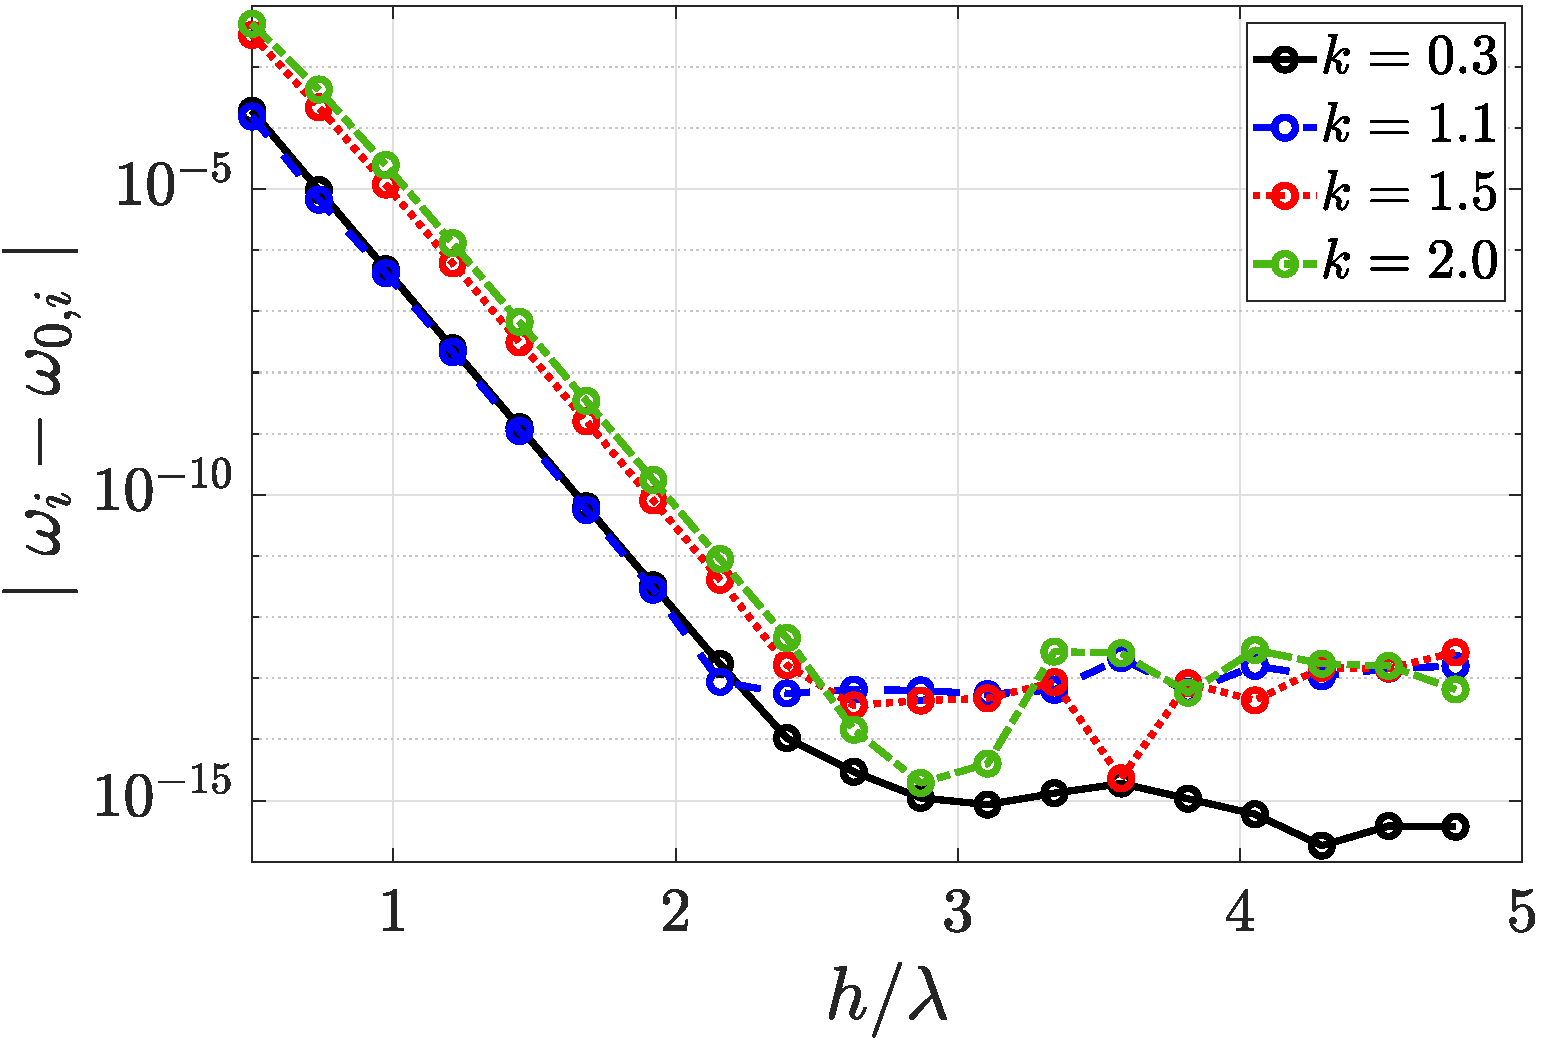
\includegraphics[width=\columnwidth]{bbc/1e3_fs}
        \caption{}
    \end{subfigure}
    \hspace{0.05\columnwidth}
    \begin{subfigure}[b]{\columnwidth}
        \centering
        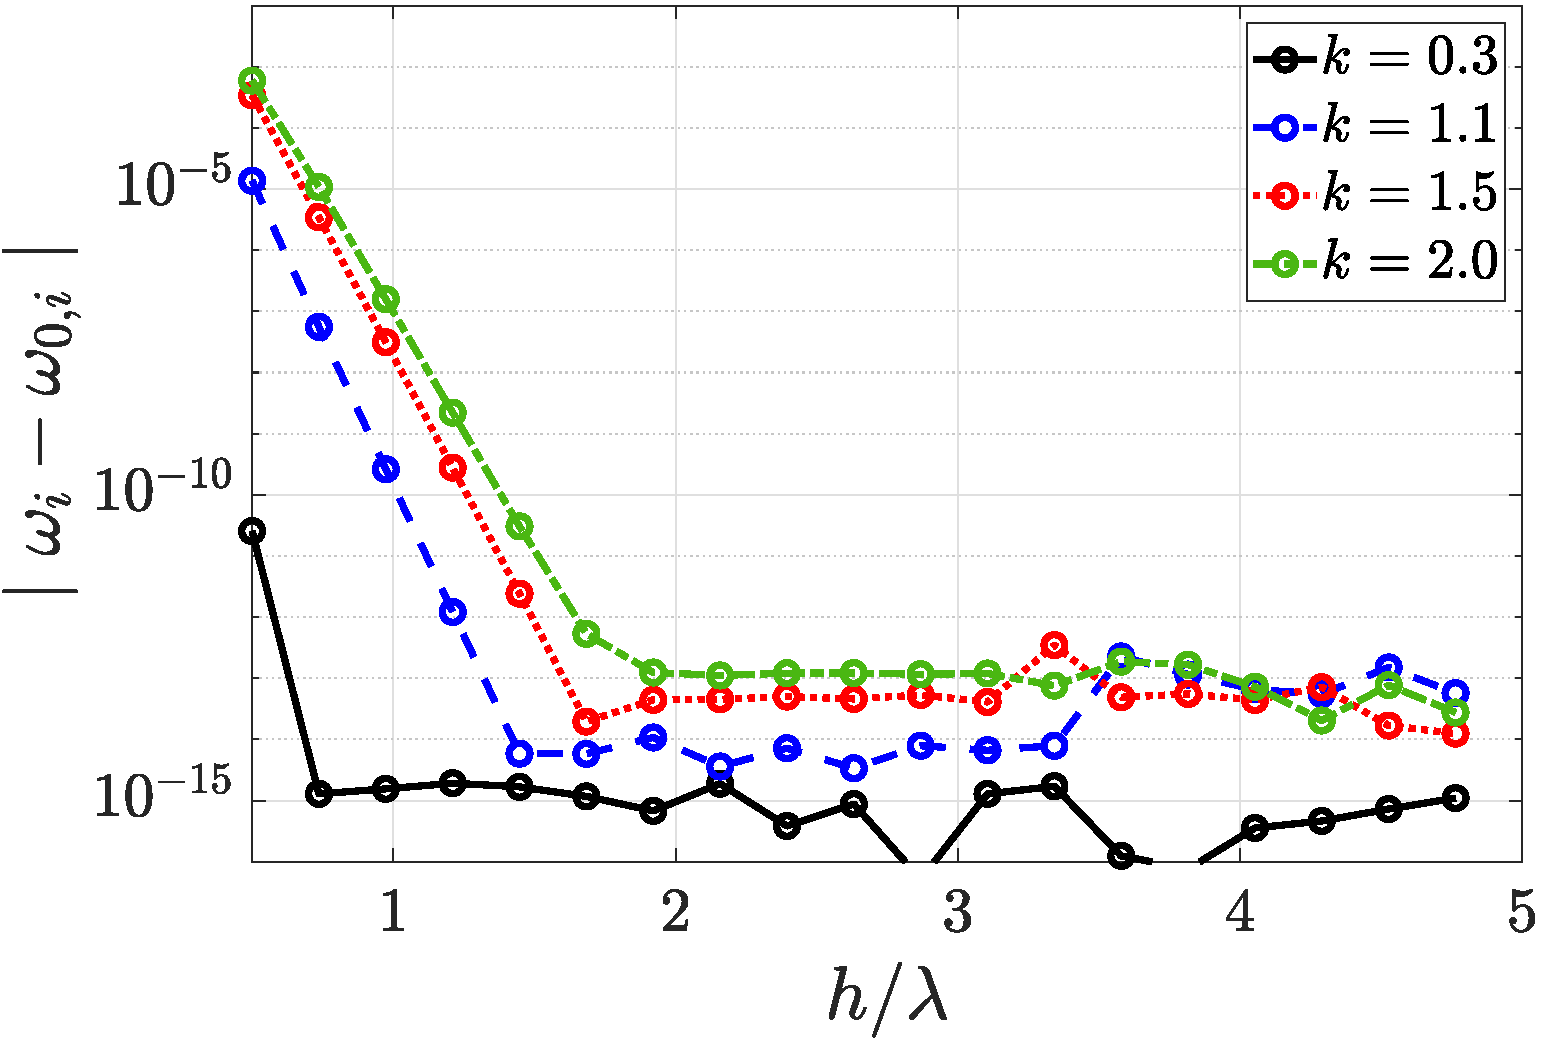
\includegraphics[width=\columnwidth]{bbc/1e3_exp}
        \caption{}
    \end{subfigure}
    \caption{Convergence of truncation height at $Re=1000$. (a) Free-slip condition, (b) Exponential decay.}
    \label{fig:h1e3}
\end{figure}
\begin{figure}[ht]
    \centering
    \begin{subfigure}[b]{\columnwidth}
        \centering
        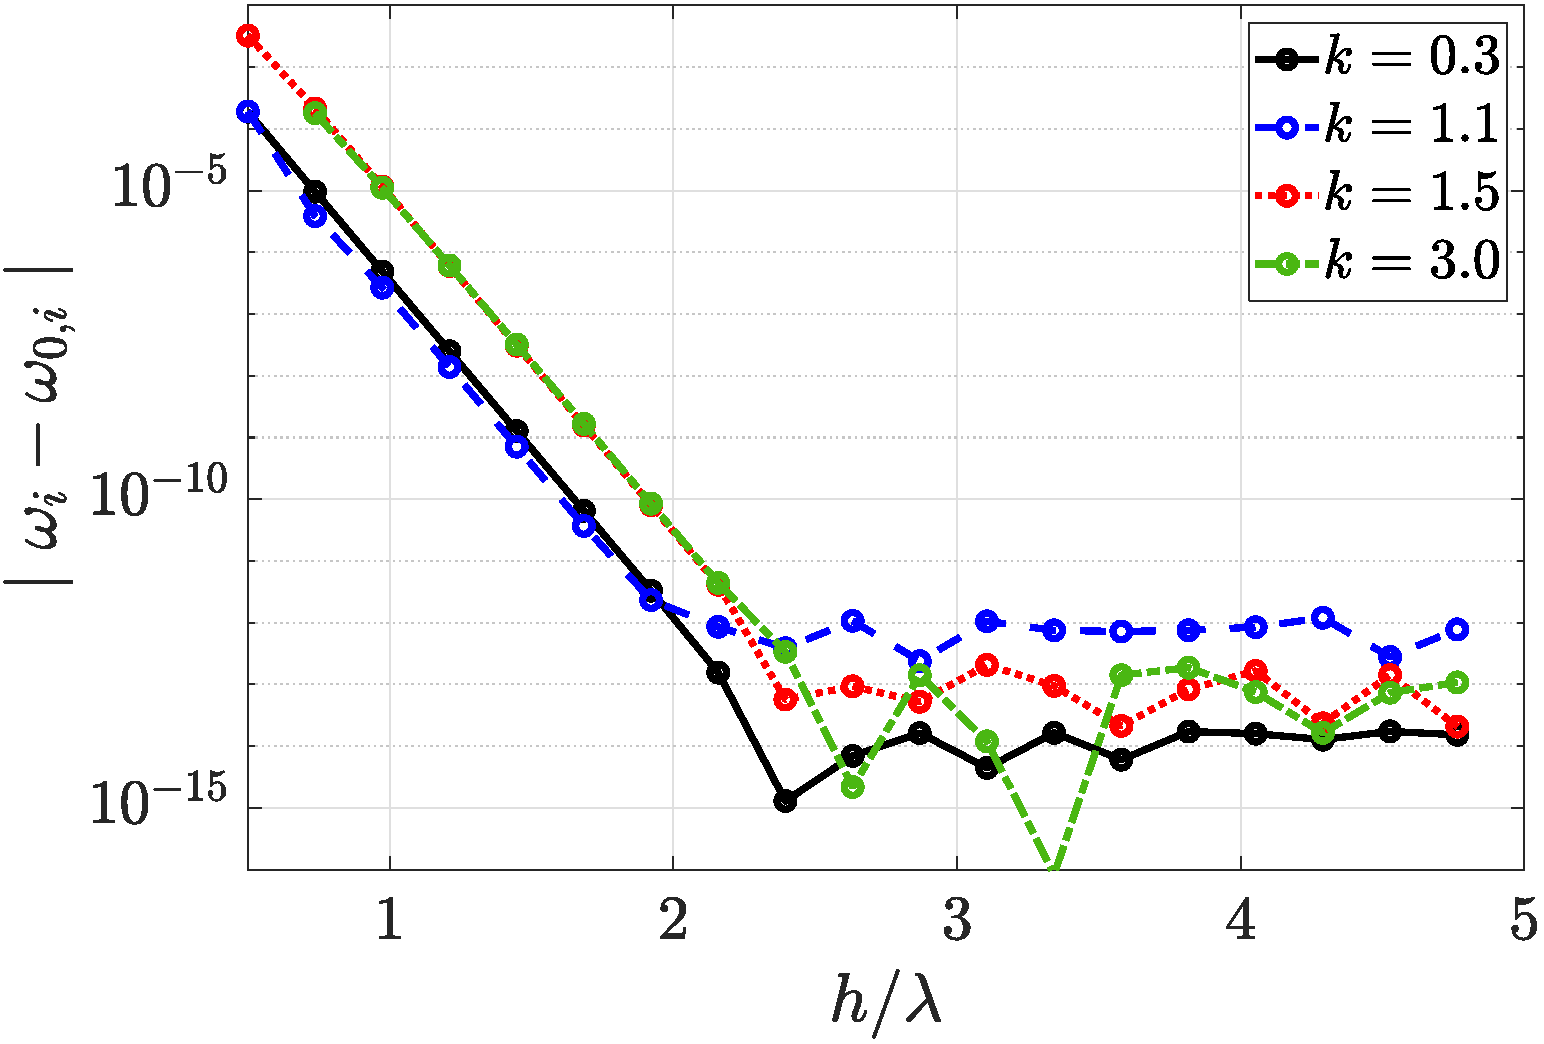
\includegraphics[width=\columnwidth]{bbc/inf_fs}
        \caption{}
    \end{subfigure}
    \hspace{0.05\columnwidth}
    \begin{subfigure}[b]{\columnwidth}
        \centering
        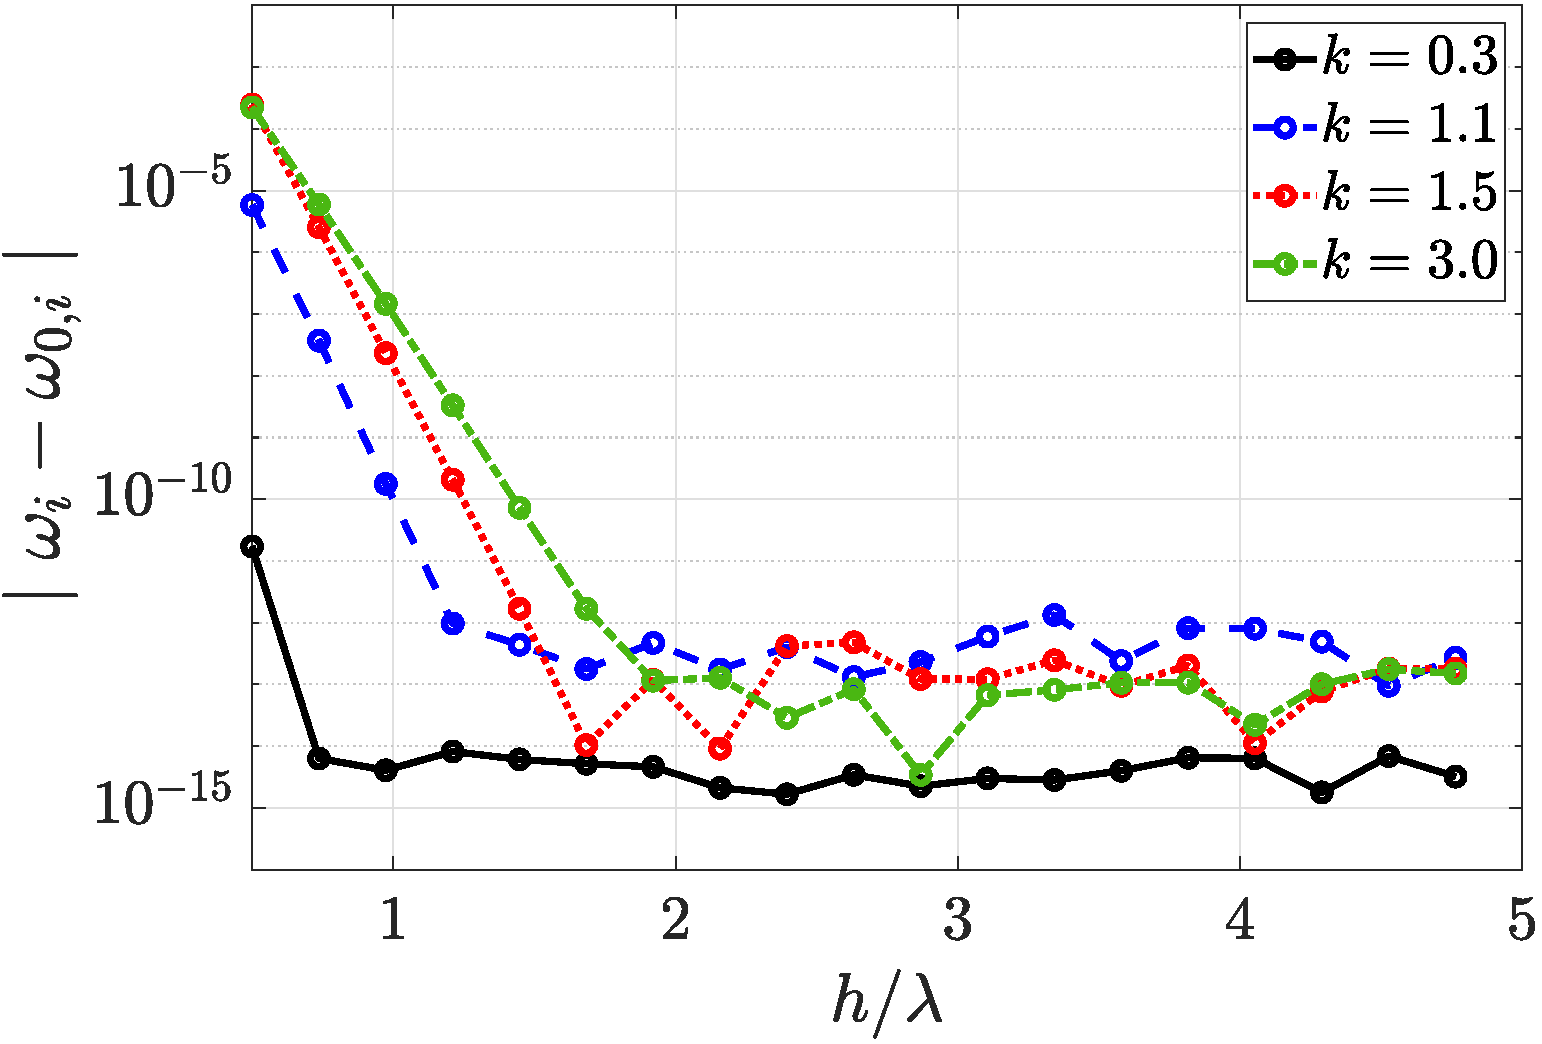
\includegraphics[width=\columnwidth]{bbc/inf_exp}
        \caption{}
    \end{subfigure}
    \caption{Convergence of truncation height at $Re=\infty$. (a) Free-slip condition, (b) Exponential decay.}
    \label{fig:hinf}
\end{figure}

\subsection{Domain decomposition method}
As described in section \ref{ch:ddm}, the domain may be split into two at the critical height, or further more split into four with two additional domains split slightly above and below the critical height. In this section the difference between the above two domain decomposition methods is analyzed, and compared with the results using the original collocation point distribution.

\begin{figure}[ht]
     \centering
     \begin{subfigure}[b]{0.48\columnwidth}
         \centering
         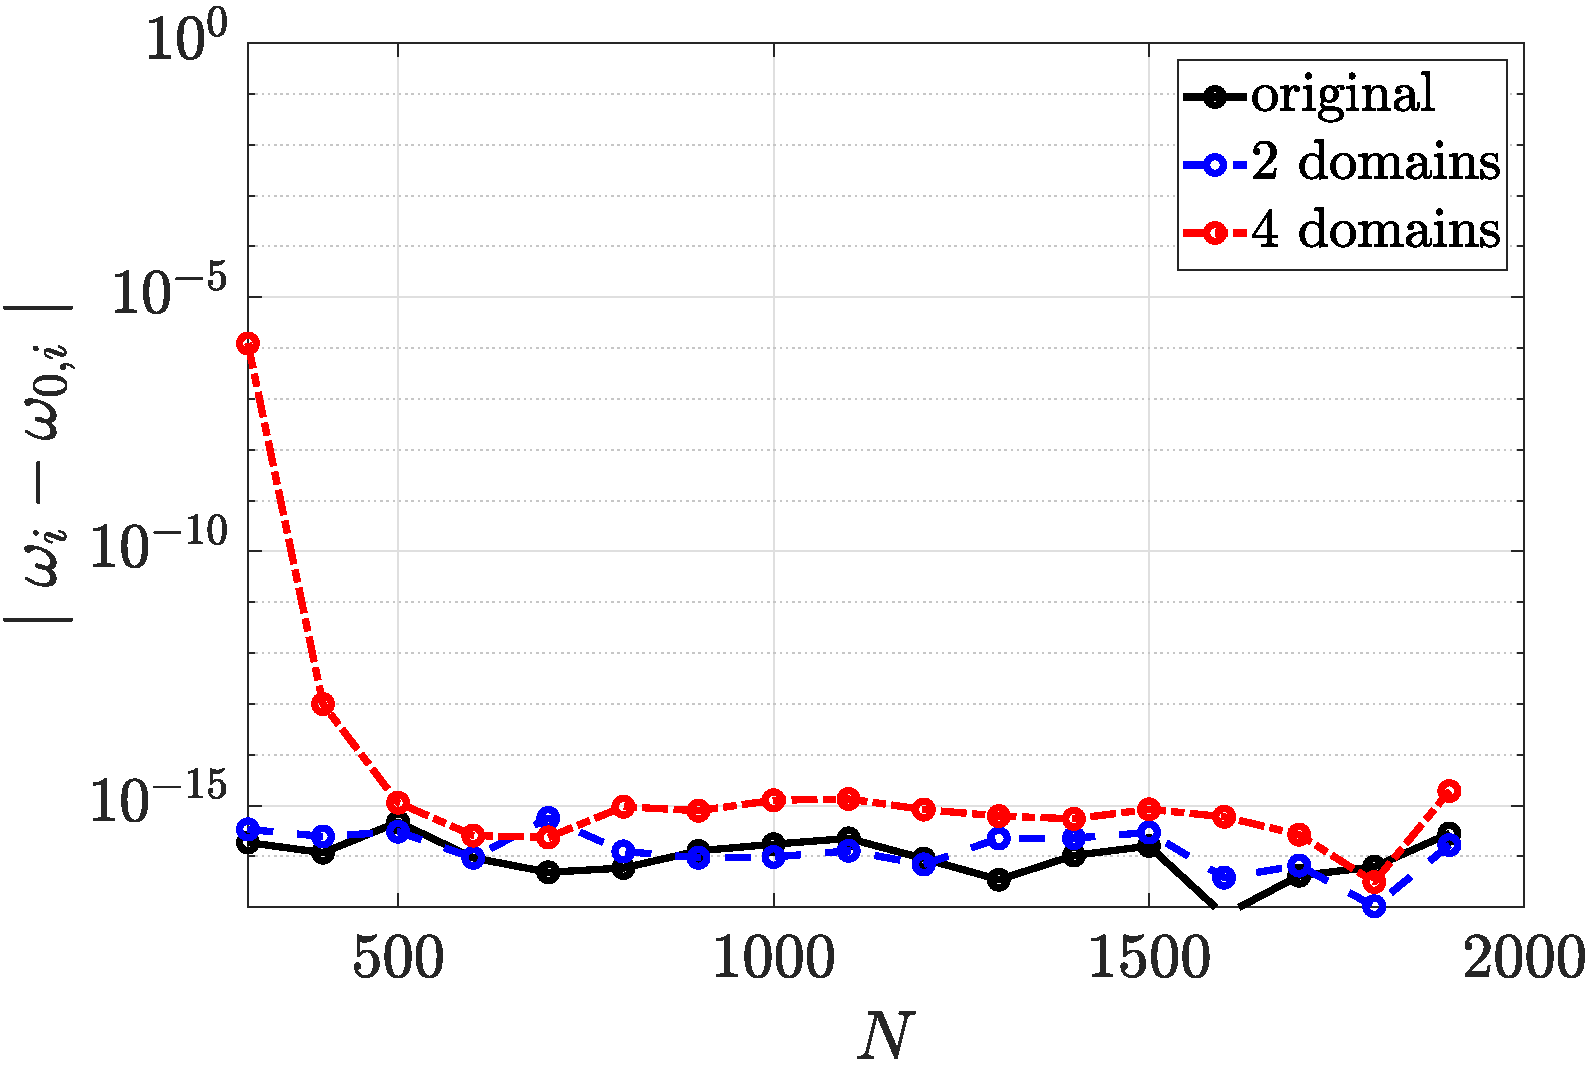
\includegraphics[width=\columnwidth]{ddm/1e3_k03}
         \caption{}
     \end{subfigure}
     \hspace{0.05\columnwidth}
     \begin{subfigure}[b]{0.48\columnwidth}
         \centering
         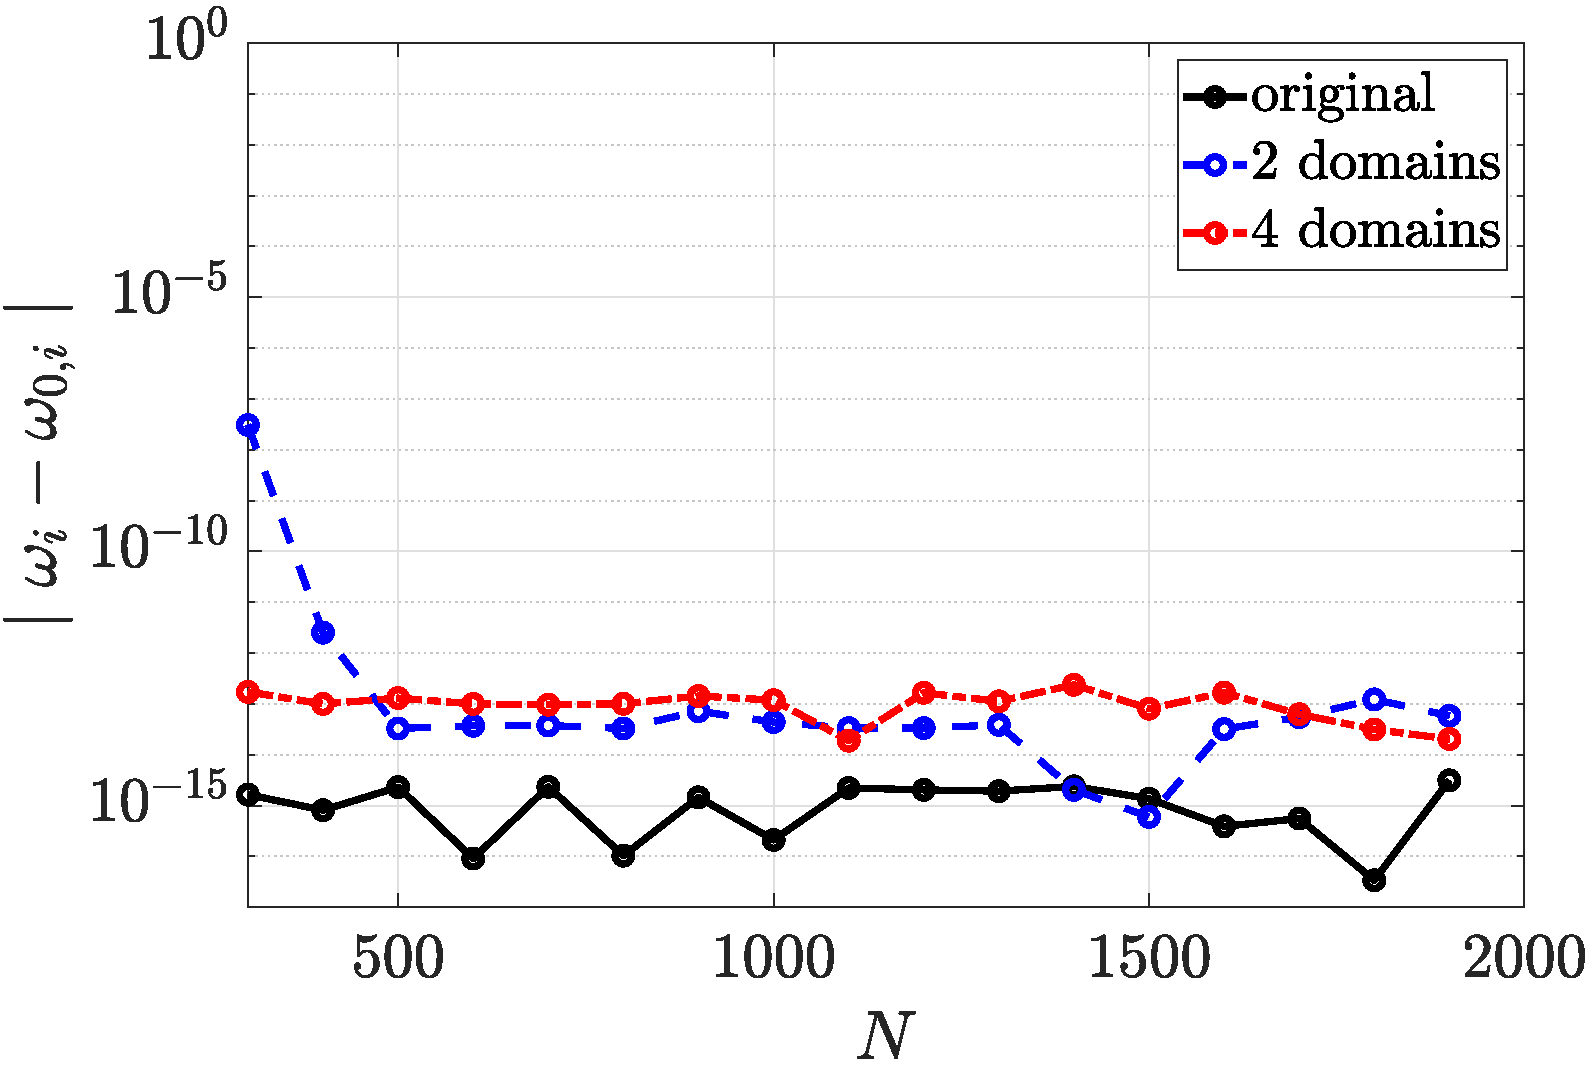
\includegraphics[width=\columnwidth]{ddm/1e3_k11}
         \caption{}
     \end{subfigure}
     \hspace{0.05\columnwidth}
     \begin{subfigure}[b]{0.48\columnwidth}
         \centering
         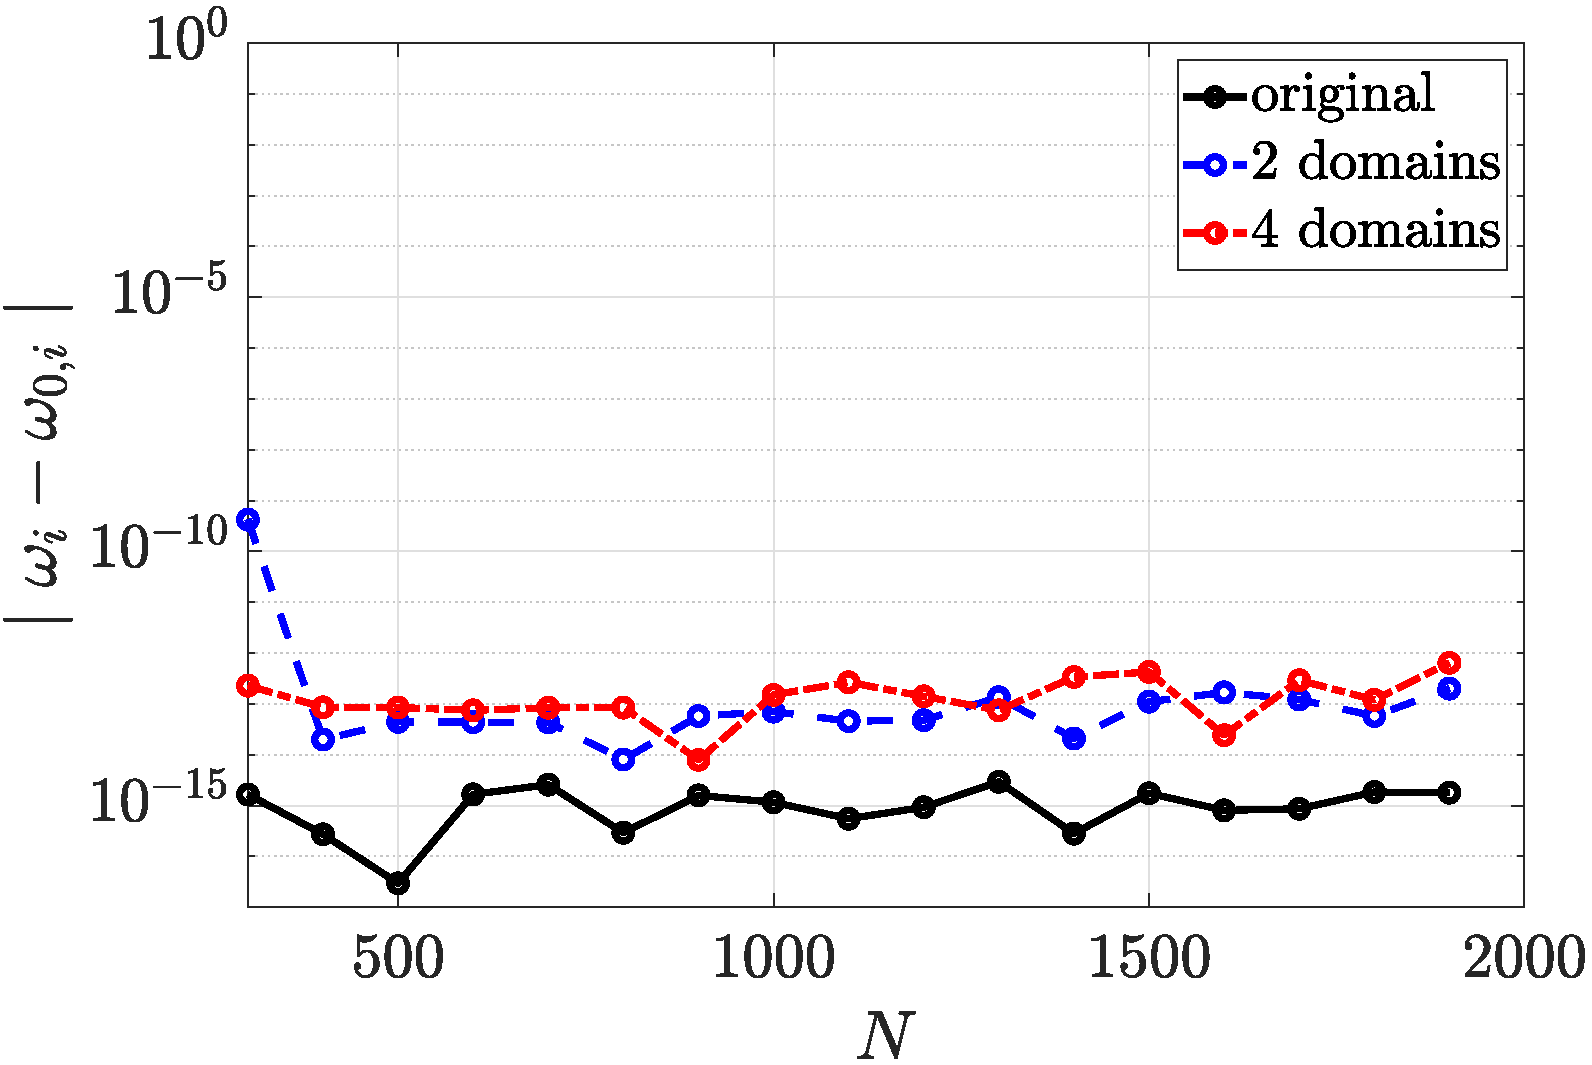
\includegraphics[width=\columnwidth]{ddm/1e3_k15}
         \caption{}
     \end{subfigure}
     \hspace{0.05\columnwidth}
     \begin{subfigure}[b]{0.48\columnwidth}
         \centering
         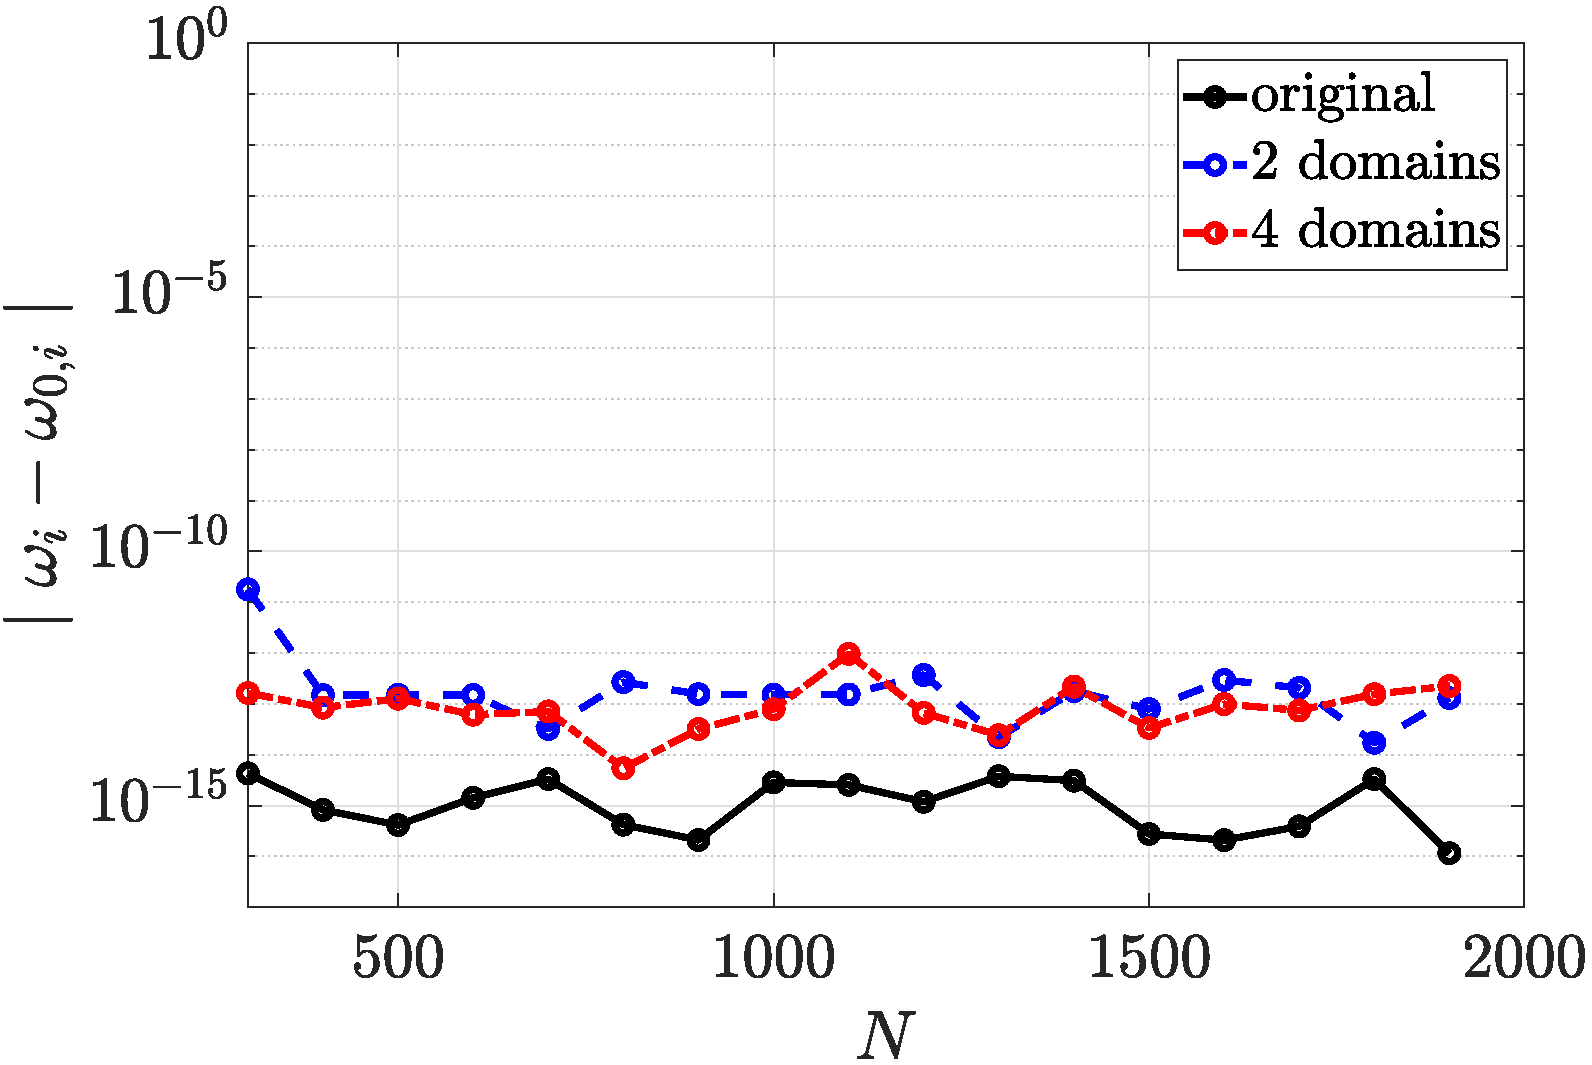
\includegraphics[width=\columnwidth]{ddm/1e3_k2}
         \caption{}
     \end{subfigure}
        \caption{Convergence of different domain decomposition methods, $Re=1000$. (a) $k=0.3$, (b) $k=1.1$, (c) $k=1.5$, (d) $k=2$.}
        \label{fig:ddm_1e3}
\end{figure}

\begin{figure}[ht]
     \centering
     \begin{subfigure}[b]{0.48\columnwidth}
         \centering
         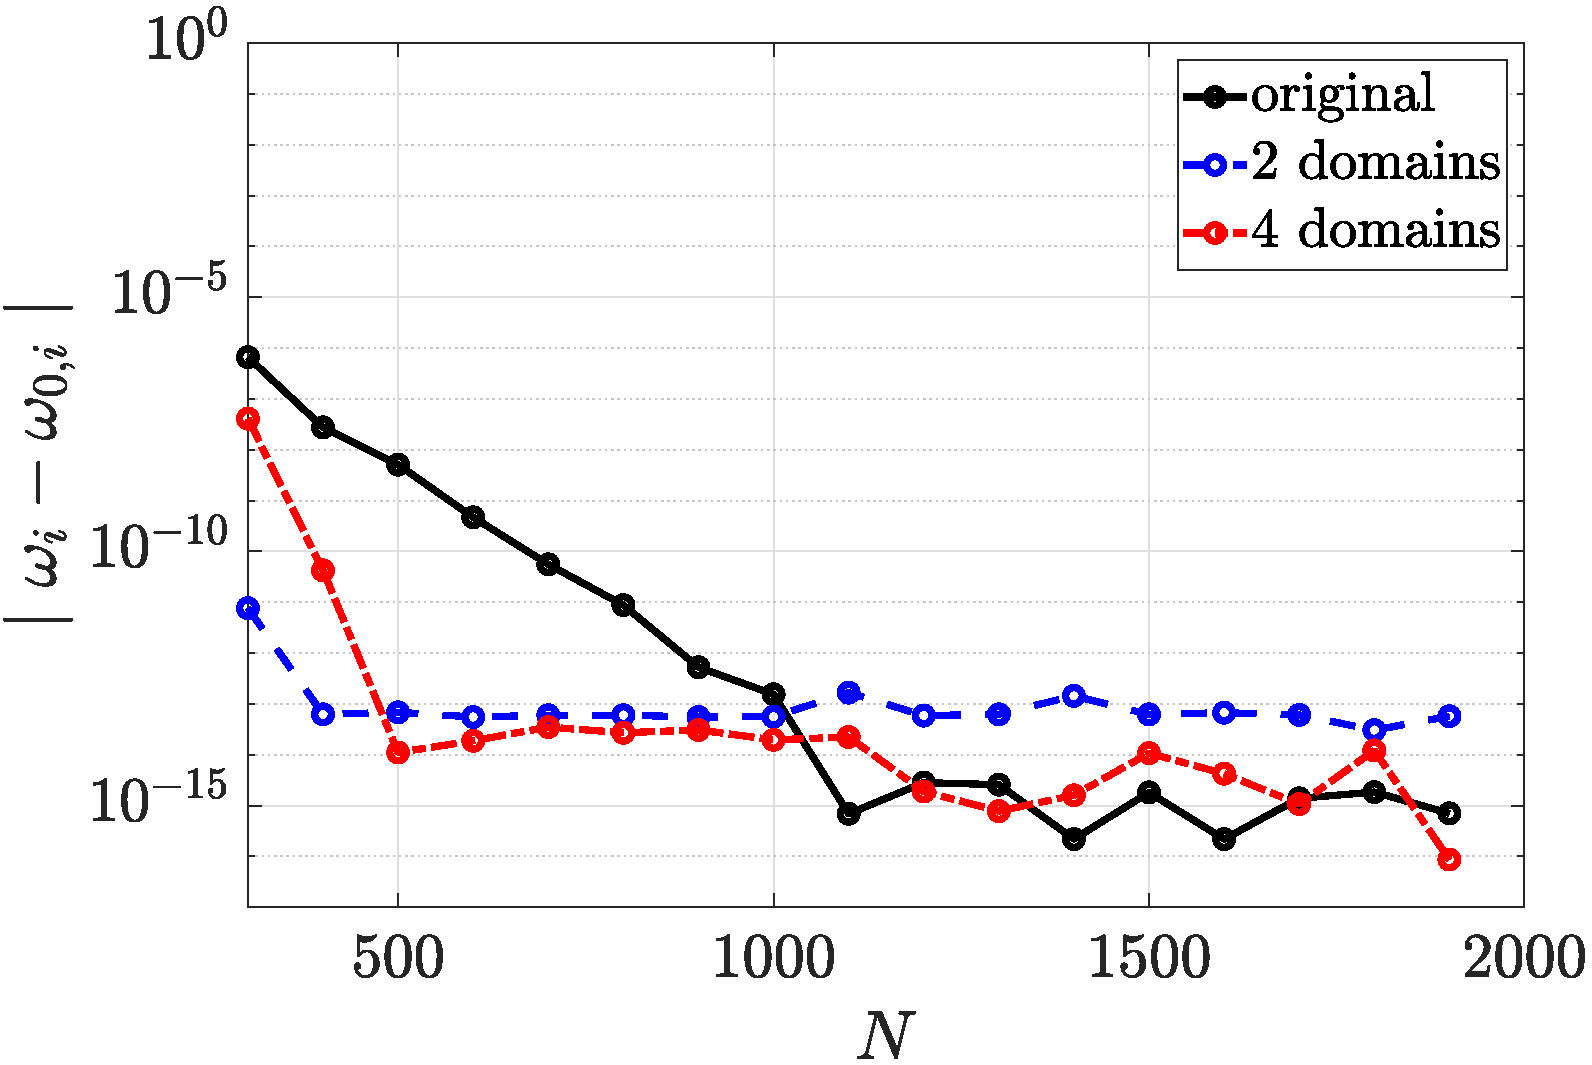
\includegraphics[width=\columnwidth]{ddm/inf_k03}
         \caption{}
     \end{subfigure}
     \hspace{0.05\columnwidth}
     \begin{subfigure}[b]{0.48\columnwidth}
         \centering
         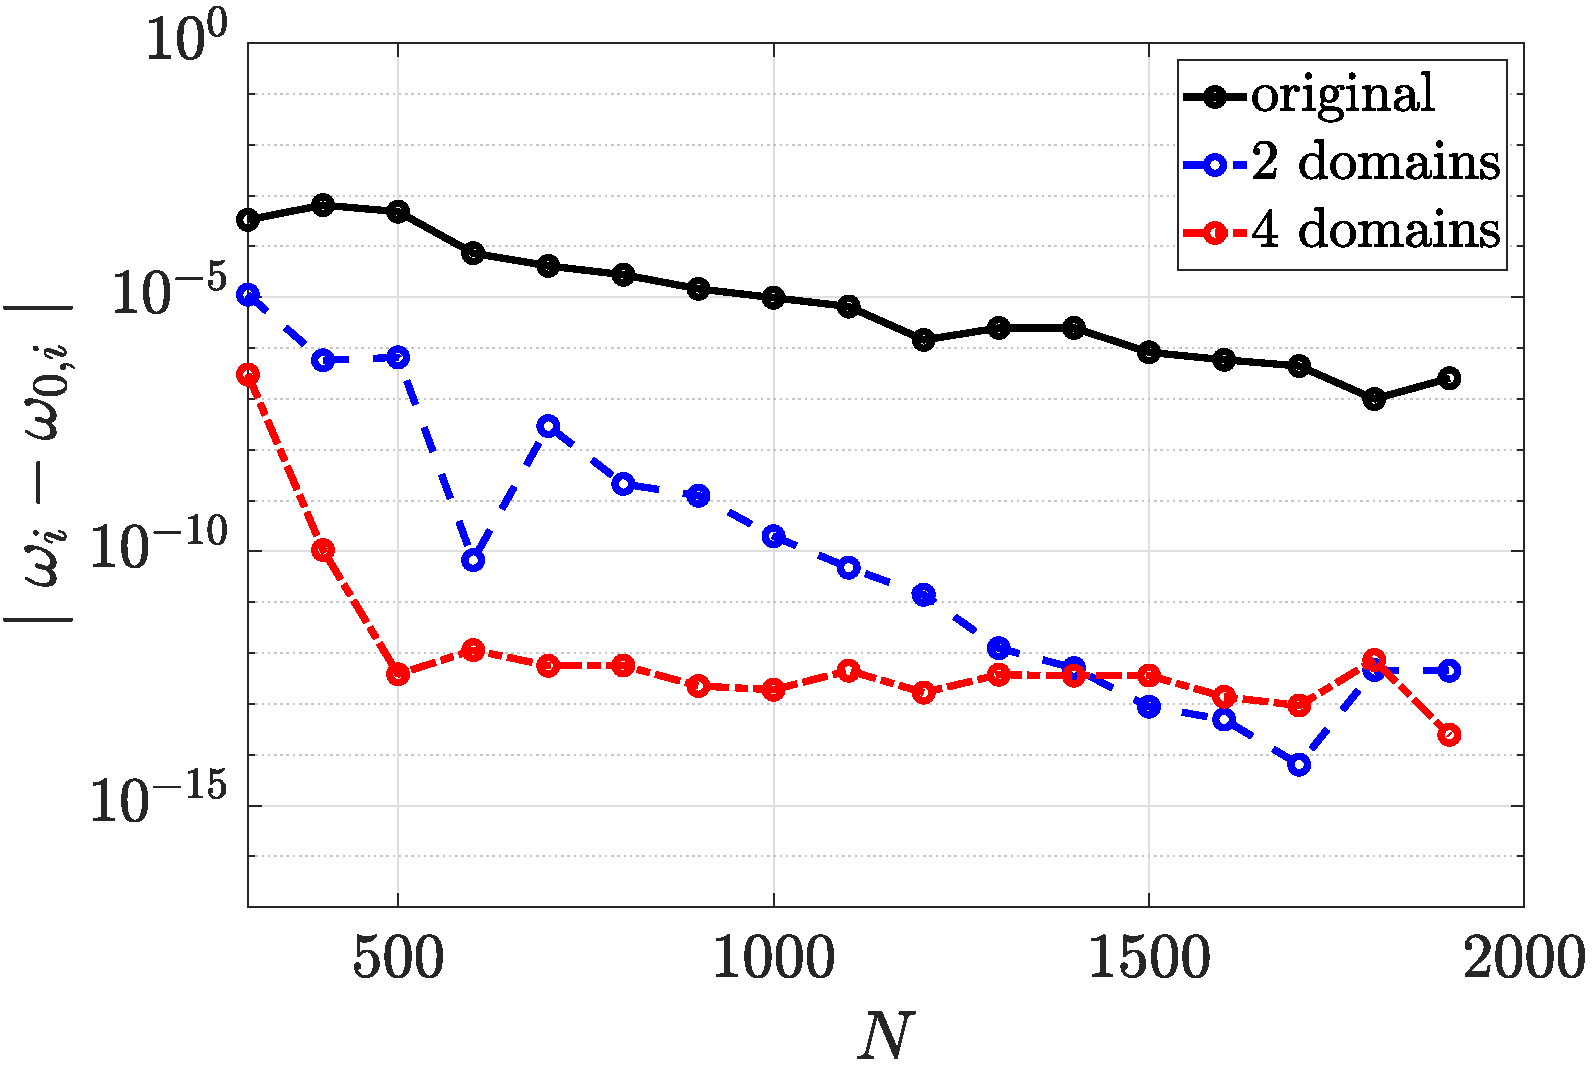
\includegraphics[width=\columnwidth]{ddm/inf_k11}
         \caption{}
     \end{subfigure}
     \hspace{0.05\columnwidth}
     \begin{subfigure}[b]{0.48\columnwidth}
         \centering
         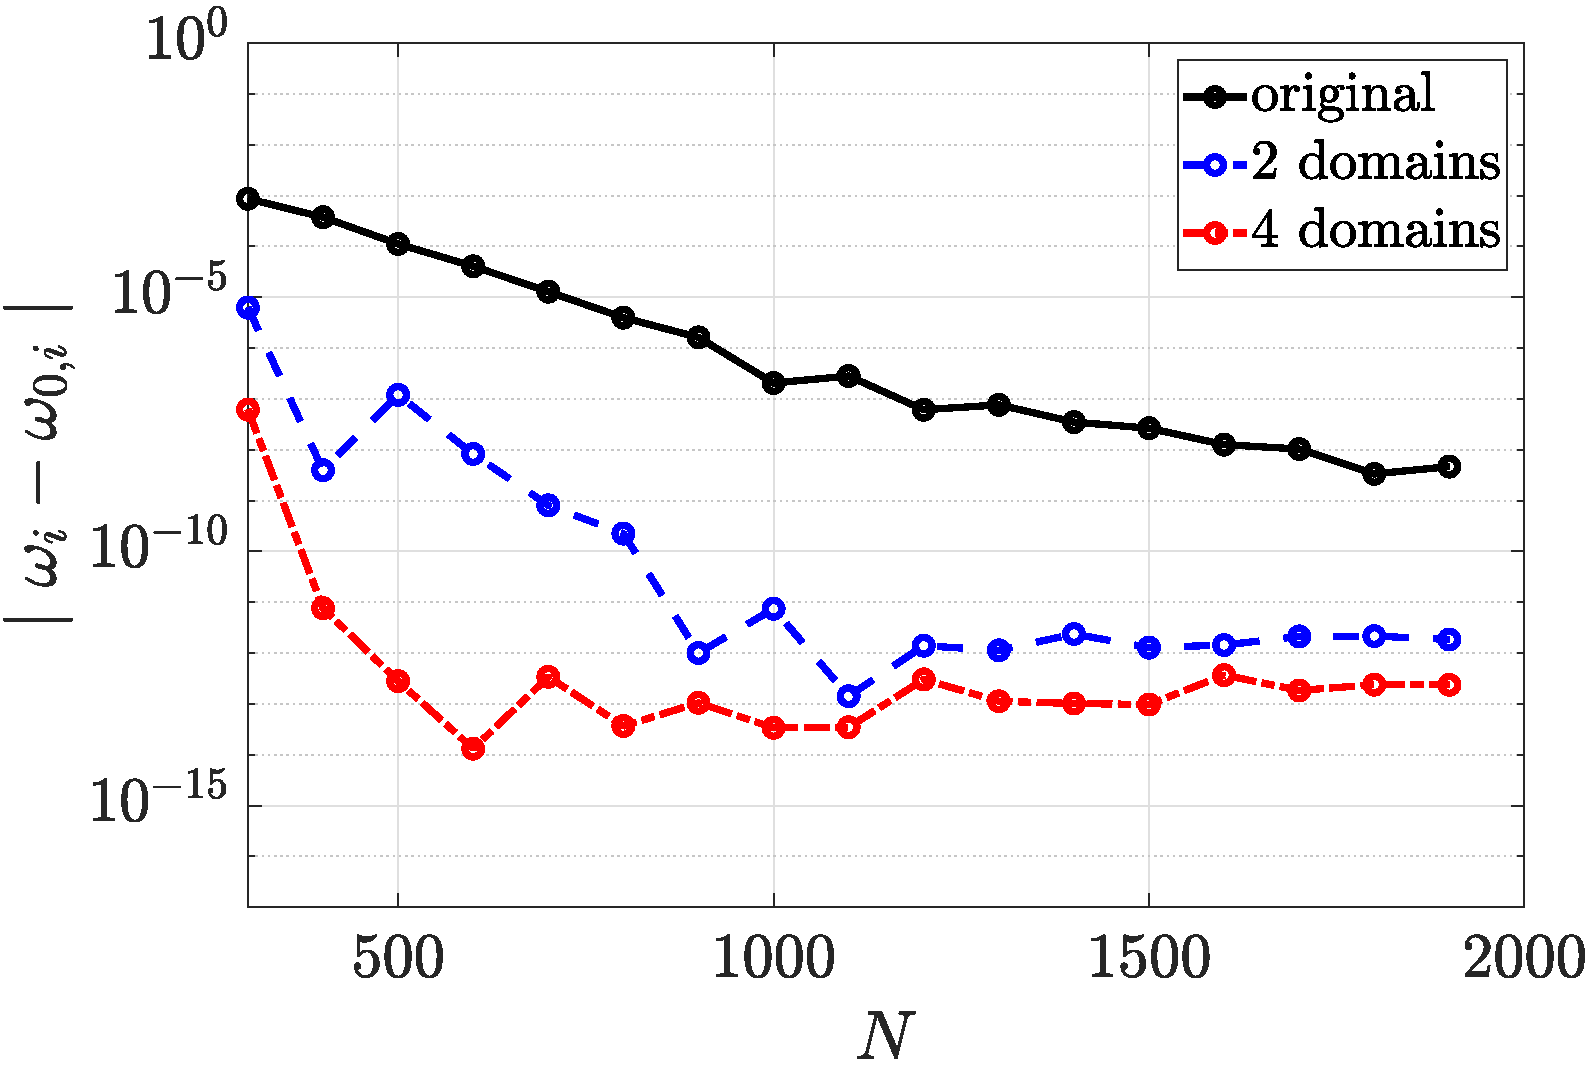
\includegraphics[width=\columnwidth]{ddm/inf_k15}
         \caption{}
     \end{subfigure}
     \hspace{0.05\columnwidth}
     \begin{subfigure}[b]{0.48\columnwidth}
         \centering
         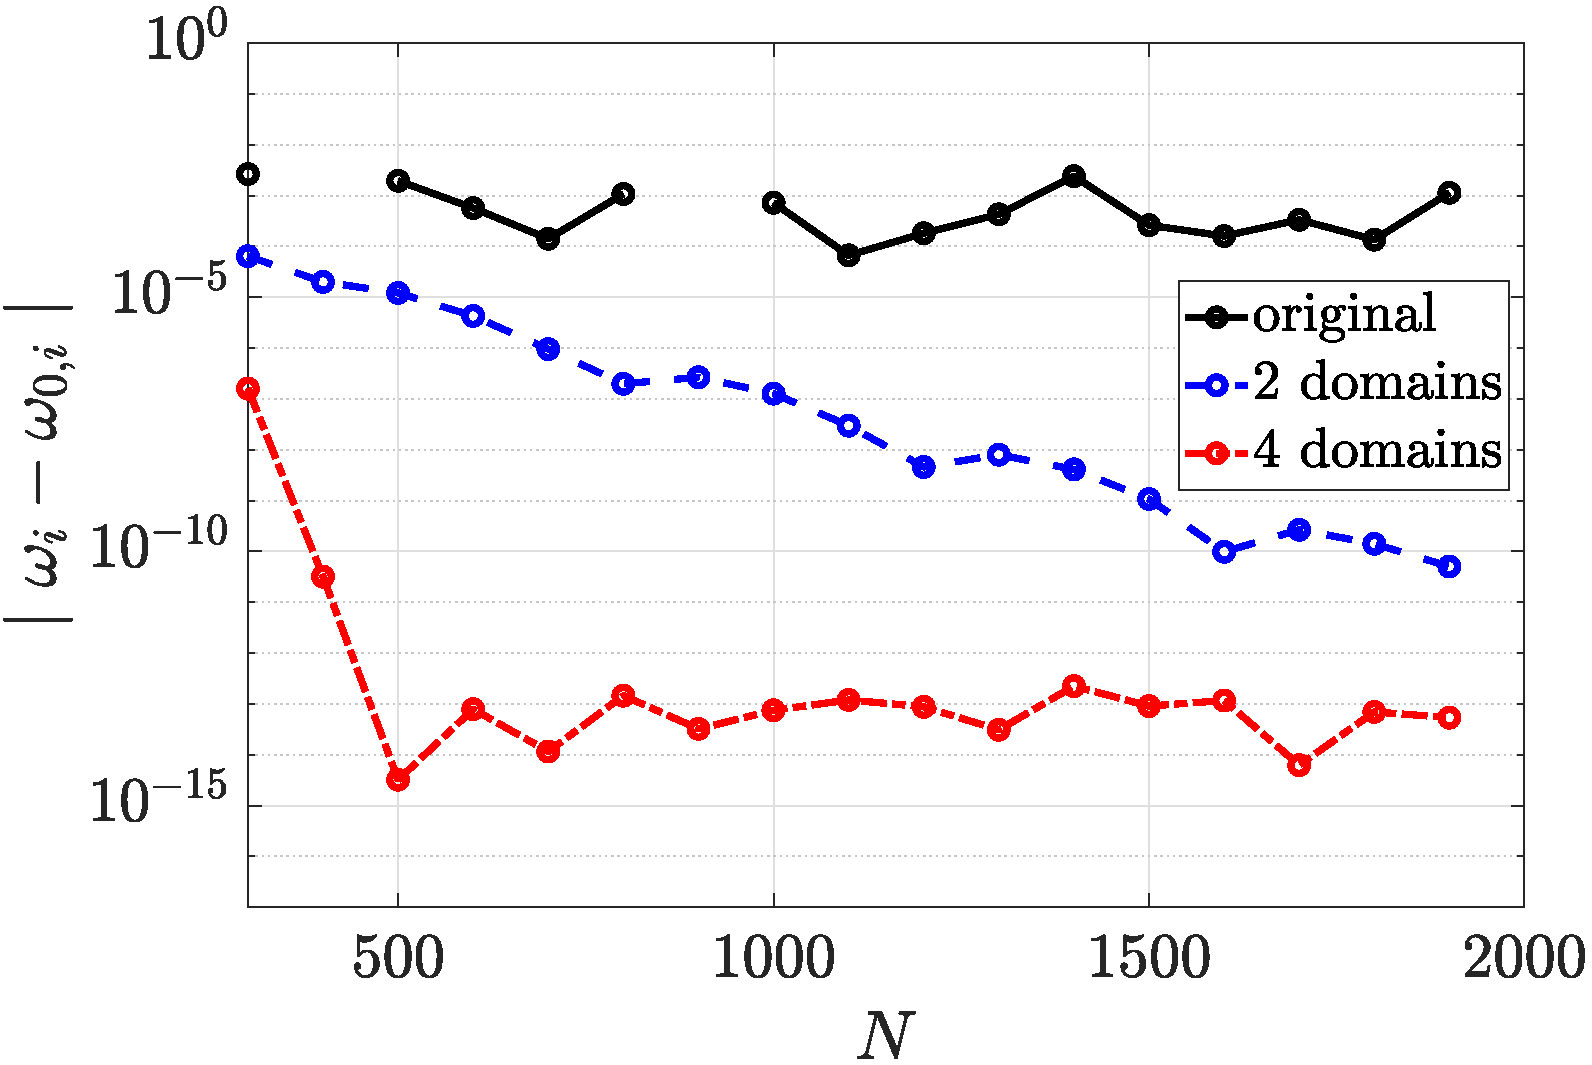
\includegraphics[width=\columnwidth]{ddm/inf_k3}
         \caption{}
     \end{subfigure}
        \caption{Convergence of different domain decomposition methods, $Re=\infty$, (a) $k=0.3$, (b) $k=1.1$, (c) $k=1.5$, (d) $k=3$.}
        \label{fig:ddm_inf}
\end{figure}


\subsection{Comparison of GEP solving algorithms}
